\chapter{Data Processing}

Lo strato del \textbf{Data Processing} è immediatamente successivo a quello della \textbf{Data Quality}: una volta che i dati sono stati puliti, formattati e adattati alle nostre esigenze, possiamo analizzarli ed elaborarli mediante l'uso di adeguati framework per poter estrarre la informazioni da dover visualizzare.\\

\section{Tecniche per il Data Processing}

\subsection{Batch Processing}

\subsection{Stream Processing} \label{StreamProc}

L'elaborazione di dati in streaming si differenzia da quella classica per il fatto che l'oggetto dell'elaborazione è un dataset unbounded, cioè un flusso di dati continuo e infinito che ha bisogno di astrazioni dedicate per applicare operatori o trasformazioni come Map, Reduce e Filter. \\

Sono possibili, in generale, 2 modelli di esecuzione con cui operare su dataset unbounded:

\begin{itemize}
    \item Streaming: elaborazione continua fintanto che vengono prodotti dati
    \item Batch: esecuzione che termina in un tempo finito, rilasciando risorse al termine
\end{itemize}

Un'esecuzione di tipo Batch è utilizzabile se non si hanno requisiti nella gestione degli stati, consumazione dei dati in-order e windowing e, quindi, generalmente, è preferibile un approccio di tipo Streaming, che prevede l'uso di un paradigma di programmazione specifico: il Dataflow Programming.

\paragraph{Dataflow Programming}  \label{DataflowProg} ~\\

Il Dataflow Programming è un paradigma di programmazione che modella un programma come un Grafo Diretto Aciclico (DAG) e si differenzia, quindi, sostanzialmente dall'Imperative Programming (o Control Flow), il quale modella un programma come una sequenza finita di operazioni. Esso, infatti, enfatizza il movimento continuo di dati tra operatori, definiti come delle Black Box con input e output espliciti usati per collegarsi con altri operatori. Visto che un operatore viene eseguito non appena tutti i suoi input sono validi, è facile notare come i linguaggi basati su questo paradigma siano inerentemente paralleli e usabili su architettura distribuite\footcite{DataflowProgramming}.

\section{Apache Spark} \label{Spark}

\section{Apache Flink}\label{Flink}

Apache Flink è un framework sviluppato per l'elaborazione continua e distribuita di flussi di dati, fondato sul paradigma del Dataflow Programming. Mette a disposizione un insieme di astrazioni utilizzabili per lo sviluppo di applicazioni:

\subsection{Livelli di astrazione}  \label{AbstractionLevels} ~\\

\begin{itemize}
	\item \textbf{Stateful Streaming}: il livello di astrazione più basso, che permette agli utenti di poter gestire liberamente il flusso di dati e la sua elaborazione, usare stati \textit{fault-tolerant} e la registrazione di callback su determinati eventi;
	\item \textbf{Core API}: è l'insieme di API base, che si divide tra \textbf{DataStream API}, per l'elaborazione di dataset bounded e unbounded, e \textbf{DataSet API}, considerato come caso particolare di un flusso di dati, usato per la sola elaborazione di dataset bounded. Queste 2 API offrono trasformazioni e operazioni come unioni, aggregazioni, windowing e gestione degli stati, necessarie per la gestione del flusso di dati considerato
	\item \textbf{Table API}: è un DSL \footnote{Domain Specific Language: un linguaggio dall'espressività limitata che si concentra su un particolare dominio.} dichiarativo che segue il modello relazionale esteso e offre la possibilità di modellare uno stream di dati come una tabella su cui effettuare proiezioni, aggregazioni, raggruppamenti e altre operazioni. Queste API risultano essere meno espressive rispetto alle Core API, ma permettono una maggiore concisione quando occorre descrivere la logica delle operazioni da eseguire sui dati.
	\item \textbf{SQL}: è il livello di astrazione più alto offerto da Flink ed interagisce con la Table API per fornire una rappresentazione dell'applicazione tramite query SQL, che possono essere eseguite sulle tabelle definite dalla Table API e, di conseguenza, direttamente sui dati.
\end{itemize}

\subsection{Flussi di dati e Programmi}  \label{ProgramsDataflows} ~\\

Gli elementi base di un'applicazione sviluppata con Flink sono, quindi:
\begin{itemize}
	\item gli \textbf{Stream}, strutture contenenti i dati
	\item gli \textbf{Operatori} di Trasformazione, che possono modificare lo stream tramite, per esempio, aggregazioni, raggruppamenti e mappature
	\item le \textbf{Source}, le fonti primarie dei dati in ingresso, file o record provenienti da code. È il nodo iniziale del DAG
	\item i \textbf{Sink}, l'output dell'applicazione, che può essere su un database, file o un processo esterno. È il nodo finale del DAG
\end{itemize}

\pagebreak

\begin{minted}{Scala}
    val lines = env.addSource(new Consumer[String](...))
	
    val events = lines.map((line) -> parse(line))
	
    val stats = events
        .keyBy("id")
        .timeWindow(Time.seconds(10))
        .apply(MyWindowAggregationFunction())
		
    stats.addSink(new RollingSink(path))
\end{minted}

\begin{figure}[th]
	\centering
	\def\svgwidth{\columnwidth}
	\input{Figures/dataflow.pdf_tex}
	\decoRule
	\caption[Streaming Dataflow]{DAG che schematizza il codice soprastante}
	\label{fig:Dataflow}
\end{figure}

\pagebreak

\paragraph{Parallelismo} \label{ParallelismFlink} ~\\

Le applicazioni scritte con Flink sono inerentemente parallele e distribuite. Durante l'esecuzione, uno Stream può avere più di una partizione, mentre ogni operatore può avere più di un sub-task che opera sui dati, ognuno indipendente dall'altro ed eseguiti su differenti thread e, se possibili, su macchine o container differenti.\\
Il parallelismo è il parametro che indica il numero di subtask che un operatore può avere e, di conseguenza, indica il numero di partizioni dello stream prodotto da quel determinato operatore.\\

\begin{figure}
    \centering
    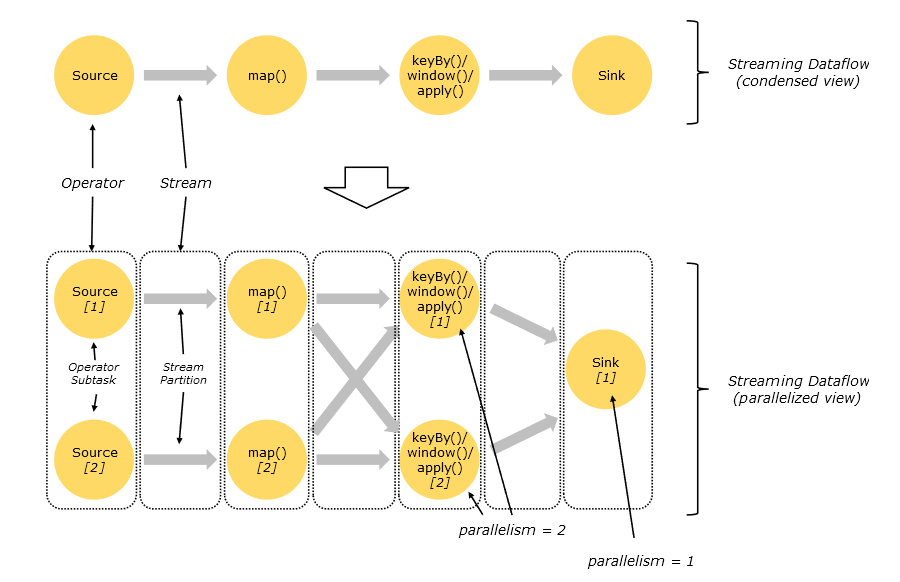
\includegraphics{Figures/parallel_dataflow.png}
    \decoRule
    \caption[Parallel Dataflow]{DAG con Parallelismo=2}
    \label{fig:ParallelDataflow}
\end{figure}

Gli Stream possono trasportare dati tra 2 operatori in base a un pattern \textit{One-to-one}, oppure a un pattern di redistribuzione (\textit{redistributing}):
\begin{itemize}
	\item Gli \textbf{\textit{stream One-to-one}} preservano il partizionamento e l'ordine degli elementi passati all'operatore. Per esempio, nell'immagine in alto, il subtask[1] dell'operatore map() vedrà gli stessi elementi, nello stesso ordine, prodotti dal subtask[1] dell'operatore Source.
    \item Gli \textbf{\textit{stream redistributing}} cambiano il partizionamento degli Stream. Ognuno dei subtask dell'operatore manda dati a diversi subtask, in base alla trasformazione che sta venendo applicata. Per esempio, l'operatore keyBy() ripartiziona lo stream usando l'hash della chiave scelta. Nel caso di stream di questo tipo, l'ordine dei dati viene preservato unicamente tra ogni coppia di subtask in comunicazione, per cui, sempre osservando l'immagine in alto, il subtask[1] di map() preserverà l'ordine con il successivo operatore keyBy(), ordine che però non è più garantito essere lo stesso
\end{itemize}

\subsection{Librerie di Flink} \label{FlinkLibs}

\subsubsection{FlinkCEP: Complex Events Processing}

FlinkCEP è una estensione di Flink che aggiunge la possibilità di effettuare analisi degli eventi in uno stream infinito di dati, grazie all'aggiunta della Pattern API. Questa API permette di specificare pattern di eventi all'interno dello stream in ingresso ed agire su di essi, innescando funzioni di Alert apposite.
\\


\begin{code}
\label{code:pattern-example}
\begin{minted}{Scala}

val input: DataStream[Event] = ...

val pattern = Pattern.begin("start").where(_.getId == 42)
.next("middle").subtype(classOf[SubEvent]).where(_.getVolume >= 10.0)
.followedBy("end").where(_.getName == "end")

val patternStream = CEP.pattern(input, pattern)

val result: DataStream[Alert] = patternStream.select(createAlert(_))
\end{minted}
\captionof{listing}{Un esempio di uso della Pattern API}
\end{code}~\\

In FlinkCEP, un \textbf{Pattern}, similmente a un pattern di un'espressione regolare, può essere \textbf{singolo} o \textbf{iterativo}. Ad esempio, nel pattern \verb|"a b+ c? d"|, \verb|a|, \verb|c?| e \verb|d| sono pattern singoli, mentre \verb|b+| è un pattern iterativo.
\\
In un Pattern possono quindi esserci, analogamente alle RegExp, Quantificatori e Condizioni.

\paragraph{Quantificatori} ~\\

I Pattern iterativi possono essere specificati usando gli appositi metodi:

\begin{itemize}
    \item \verb|pattern.oneOrMore()|, per pattern in cui si aspetta una o più occorrenze di un dato evento;
    \item \verb|pattern.times(#ofTimes)|, per pattern in cui ci si aspetta un evento ripetuto un numero fisso di volte;
    \item \verb|pattern.optional()|, utilizzabile per tutti i tipi di Pattern per renderli opzionali
\end{itemize}

\paragraph{Condizioni} ~\\

Per ogni pattern, è possibile specificare condizioni aggiuntive, che possono essere legate alla proprietà di un certo evento in arrivo, oppure alla contiguità di eventi che soddisfano certe condizioni.

Per questo, usando i metodi \verb|pattern.where()| e \verb|pattern.or()| è possibile specificare delle \verb|IterativeCondition|s, \verb|SimpleCondition|s oppure una combinazione di più condizioni.
\\
Alcuni esempi:

\begin{code}
\label{code:iterative-cond}
\begin{minted}{Scala}
middle.oneOrMore().where(
    (value, ctx) => {
        lazy val sum = ctx.getEventsForPattern("middle")
                          .asScala.map(_.getPrice).sum
        value.getName.startsWith("foo") && sum + value.getPrice < 5.0
    }
)
\end{minted}
\captionof{listing}{Iterative Condition}
\end{code}~\\

\begin{code}
    \label{code:simple-cond}
    \begin{minted}{Scala}
start.where(event => event.getName.startsWith("foo"))

start.subtype(classOf[SubEvent]).where(subEvent => ... /* some condition */)


    \end{minted}
    \captionof{listing}{Iterative Condition}
\end{code}~\\

\subsubsection{Flink Gelly: Graph Processing}

\subsubsection{FlinkML: Machine Learning}


